\chapter{Introduction}\label{ch:introduction}
\todo{All our code files should be in appendix, call it "Source code" and list all the files}
\todo{Do we refer to Queue and Stack functions? It should be in the appendix a code anyways}
\todo{Block diagram is missing in appendix, and does it get referred to in the text?}

This report documents the development of a path-finding robot,
with the purpose of bettering the groups understanding of computation on a microprocessor based platform.

The set goal of the robot was to be able to find the most efficient way
from a given starting point to a given destination on any map.
The idea for this project stems from rescue situations,
where it would be unsafe for a human rescuer to enter the area.

In order to make this feasible within the time limits of this project,
we adapted the RoboCup Junior Rescue rules \cite{Robocup} into specific limitations.
These are rules for a competition for high school students,
where the goal is to educate about building robots.
The focus here is set on rescuing robots,
but there are also other RoboCup competitions with different topics.

Those limitations are mainly about the map and surface,
and have been altered slightly,
to fit the semesters requirements and account for the size of our group.

Analysing the problem showed us,
that our high level requirements for a rescue robot were:
movability,
knowing where the robot is,
reacting to a changing environment and
calculating a path.
We defined limits for these required fields, as can be seen in Table \ref{tab:limits},
to make it possible for us to develop a satisfying result in the time of the project. 

\begin{table}[h]
\centering
\begin{tabular}{|l|l|}
	\hline%----------------------
	Field 				& Limits							\\
	\hline%----------------------
	Movability			& Even terrain						\\
	Placement			& Limited map, known size			\\
	Reaction to a changing environment	& Limited change allowed			\\
	Path Calculation	& Map can be approximated as a grid	\\
	\hline%----------------------
\end{tabular}
\caption{Delimitations for the defined Fields of Focus}
\label{tab:limits}
\end{table}

\begin{figure}[!ht]
	\centering
	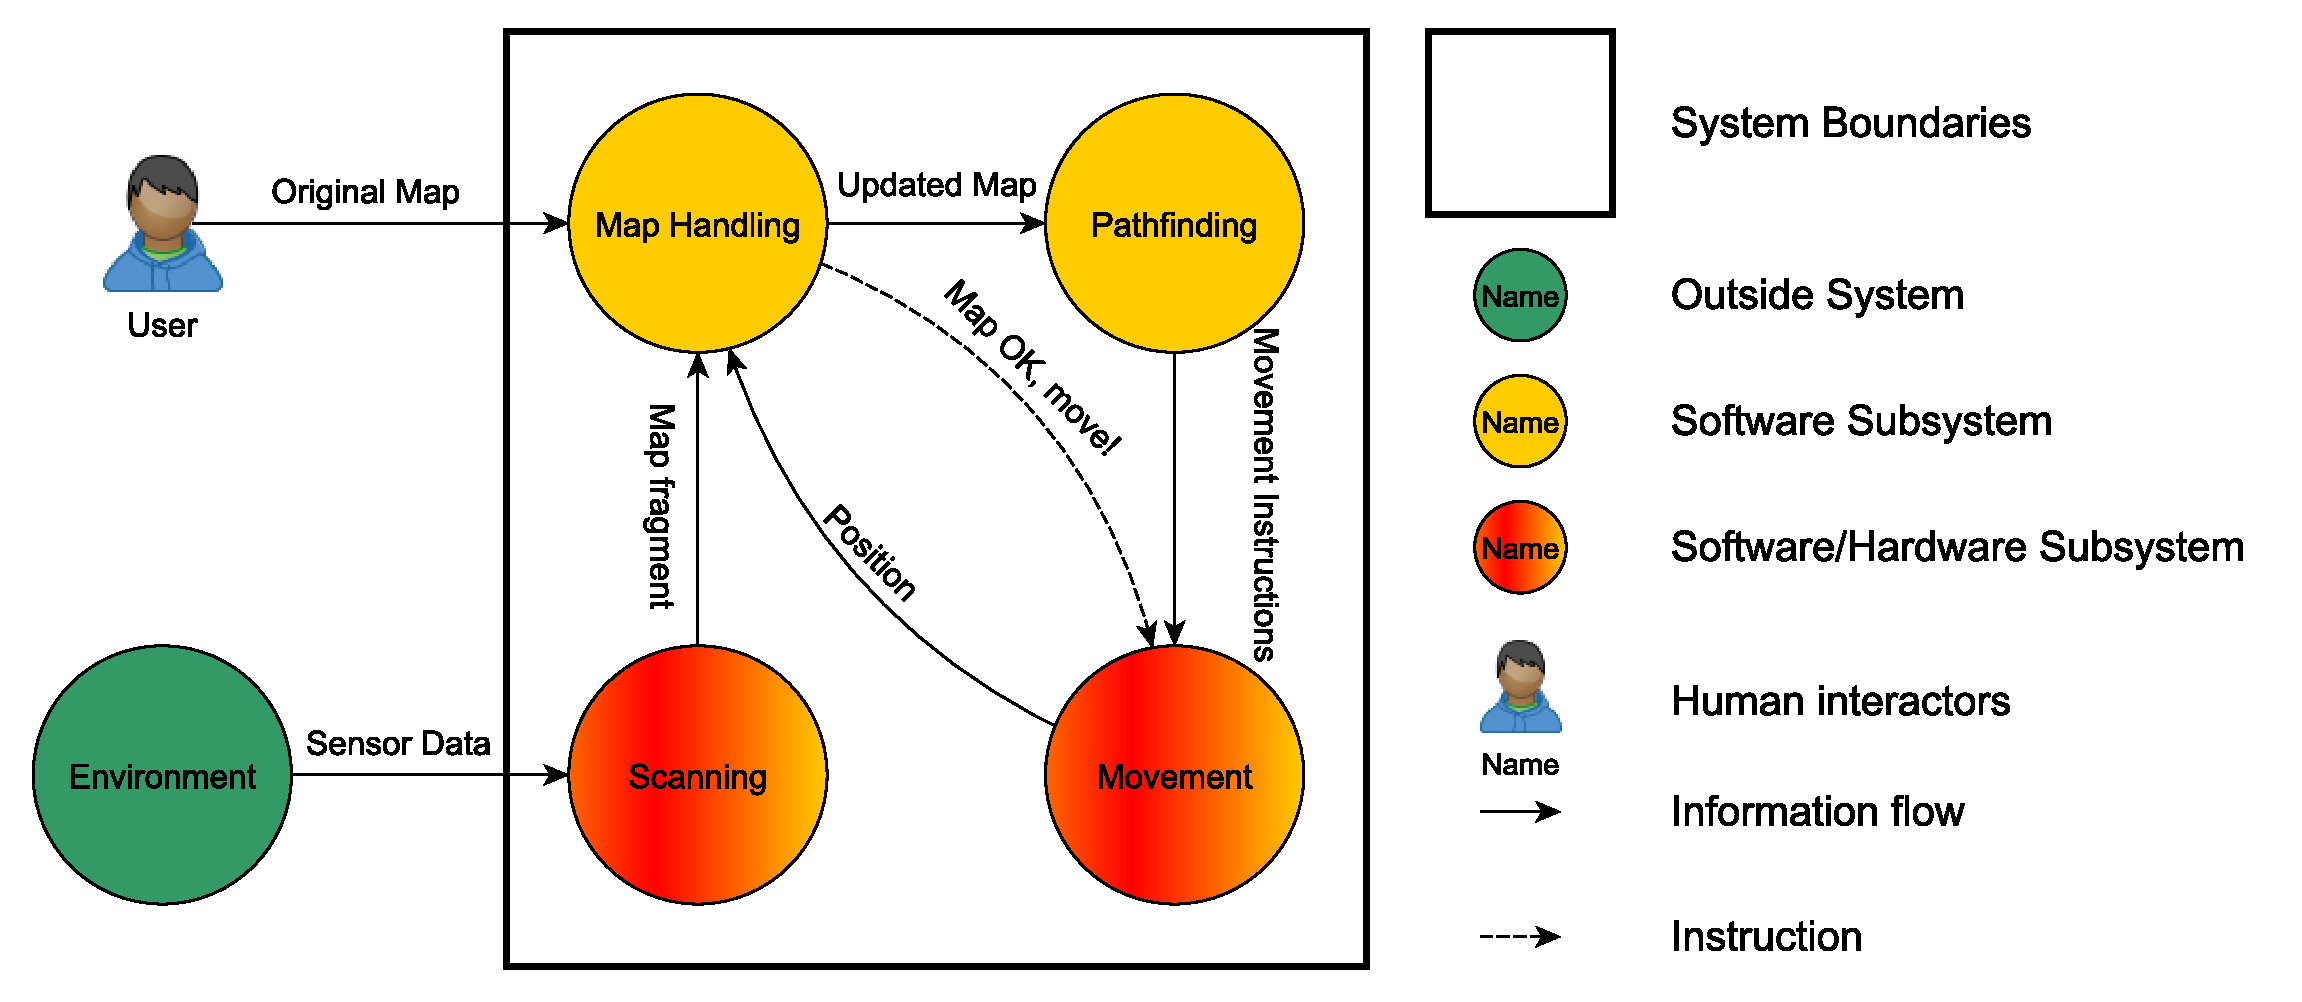
\includegraphics[width=\textwidth]{figures/intro/systemview}
	\caption{Information-Flow diagram of Robot Subsystems}
	\label{fig:system} 
\end{figure}
After analysing the problem,
we came to the conclusion,
that a modular system,
as described in Figure \ref{fig:system},
would fit our needs best.

Based on the knowledge we got from the book
"Object-Oriented Systems Analysis and Design  Using UML" \cite{Benett2010},
we decided to define our system with logical subsystems.
This allowed us to handle the different sections of the environment independently,
and makes future changes more feasible.
It also makes it possible to individually test the subsystems,
while other systems may not work yet.
We defined four subsystems, each handling one of the high level requirements,
mentioned earlier in Table \ref{tab:limits}.
Two of those have to handle inputs from the environment (\emph{Scanning} and \emph{Map Handling}),
the other two only get inputs from inside the system.

Modularising a system makes simultaneous development
and independent testing possible.
Our approach created two pure software systems,
the other two are a mixture of software and hardware.

We had some issues with acquiring the needed hardware,
but thanks to subdivision,
we were still able to develop and test the software subsystems.

\subsection*{Reading Guide}
The chapters in this report are to be understood as explanations of the previously mentioned subsystems.\\
Chapter \ref{ch:map_handling} covers how the changing environment is handled.
It contains a detailed view of requirements and map design,
as well as an in depth discussion of our implementation.
Chapter \ref{ch:move} gives an introduction to stepper motors, explains the type of wheels used and goes into detail about the custom built circuit used for controlling the direction.
Chapter \ref{ch:scan} introduces the used sensors and 
explains how their values get combined to be further useful in the other subsystems.
Chapter \ref{ch:path} covers basic graph theory,
develops an understanding of different path-finding algorithms,
explains the reasons to chose a specific algorithm in our context and
goes into detail about the programmatic implementation.

